\documentclass[12pt,t]{beamer}
\usepackage{graphicx}
\setbeameroption{hide notes}
\setbeamertemplate{note page}[plain]

% get rid of junk
\usetheme{default}
\beamertemplatenavigationsymbolsempty
\hypersetup{pdfpagemode=UseNone} % don't show bookmarks on initial view

% font
\usepackage{fontspec}
\setsansfont{TeX Gyre Heros}
\setbeamerfont{note page}{family*=pplx,size=\footnotesize} % Palatino for notes
% "TeX Gyre Heros can be used as a replacement for Helvetica"
% In Unix, unzip the following into ~/.fonts
% In Mac, unzip it, double-click the .otf files, and install using "FontBook"
%   http://www.gust.org.pl/projects/e-foundry/tex-gyre/heros/qhv2.004otf.zip

% named colors
\definecolor{offwhite}{RGB}{249,242,215}
\definecolor{foreground}{RGB}{255,255,255}
\definecolor{background}{RGB}{24,24,24}
\definecolor{title}{RGB}{107,174,214}
\definecolor{gray}{RGB}{155,155,155}
\definecolor{subtitle}{RGB}{102,255,204}
\definecolor{hilight}{RGB}{102,255,204}
\definecolor{vhilight}{RGB}{255,111,207}
\definecolor{lolight}{RGB}{155,155,155}
%\definecolor{green}{RGB}{125,250,125}

% use those colors
\setbeamercolor{titlelike}{fg=title}
\setbeamercolor{subtitle}{fg=subtitle}
\setbeamercolor{institute}{fg=gray}
\setbeamercolor{normal text}{fg=foreground,bg=background}
\setbeamercolor{item}{fg=foreground} % color of bullets
\setbeamercolor{subitem}{fg=gray}
\setbeamercolor{itemize/enumerate subbody}{fg=gray}
\setbeamertemplate{itemize subitem}{{\textendash}}
\setbeamerfont{itemize/enumerate subbody}{size=\footnotesize}
\setbeamerfont{itemize/enumerate subitem}{size=\footnotesize}

% page number
\setbeamertemplate{footline}{%
    \raisebox{5pt}{\makebox[\paperwidth]{\hfill\makebox[20pt]{\color{gray}
          \scriptsize\insertframenumber}}}\hspace*{5pt}}

% add a bit of space at the top of the notes page
\addtobeamertemplate{note page}{\setlength{\parskip}{12pt}}

% a few macros
\newcommand{\bi}{\begin{itemize}}
\newcommand{\ei}{\end{itemize}}
\newcommand{\ig}{\includegraphics}
\newcommand{\subt}[1]{{\footnotesize \color{subtitle} {#1}}}


% title info
\title{Data structures}
\author{Bjarki Ágúst Guðmundsson \\ Tómas Ken Magnússon}
\institute{\href{http://ru.is/td}{School of Computer Science} \\[2pt] \href{http://ru.is}{Reykjavík University}}
\date{Árangursrík forritun og lausn verkefna}
% \date{\href{http://www.biostat.wisc.edu/~kbroman}{\tt \scriptsize biostat.wisc.edu/{\textasciitilde}kbroman}
% \\[-4pt]
% \href{http://github.com/kbroman}{\tt \scriptsize github.com/kbroman}
% }


% Tikz
\usepackage{tikz}
\usetikzlibrary{arrows,shapes}

% Minted
\usepackage{minted}
\usemintedstyle{monokai}
\newminted{cpp}{fontsize=\footnotesize}

% Graph styles
\tikzstyle{vertex}=[circle,fill=black!50,minimum size=15pt,inner sep=0pt, font=\small]
\tikzstyle{selected vertex} = [vertex, thick, draw=vhilight]
\tikzstyle{edge} = [draw,thick,-]
\tikzstyle{dedge} = [draw,thick,->]
\tikzstyle{weight} = [font=\scriptsize,pos=0.5]
\tikzstyle{selected edge} = [draw,line width=2pt,-,red!50]
\tikzstyle{ignored edge} = [draw,line width=5pt,-,black!20]


\begin{document}

% title slide
{
    \setbeamertemplate{footline}{} % no page number here
    \frame{
        \titlepage
    }
}


\begin{frame}{Today we're going to cover}
    \vspace{40pt}
    \bi
        \item Review the Union-Find data structure, and look at applications
        \item Study range queries
        \item Learn about Segment Trees
        % \item Learn about Fenwick Trees
    \ei
\end{frame}

% TODO: Union-Find
\begin{frame}[fragile]{Union-Find}
    \vspace{20pt}
    \bi
        \item We have $n$ items
        \item Maintains a collection of disjoint sets
        \item Each of the $n$ items is in exactly one set
        \vspace{10pt}
        \item $items = \{1,2,3,4,5,6\}$
        \item $collections = \{1,4\}, \{3,5,6\}, \{2\}$
        \item $collections = \{1\}, \{2\}, \{3\}, \{4\}, \{5\}, \{6\}$
        \vspace{10pt}
        \item Supports two operations efficiently: \texttt{find(x)} and \texttt{union(x,y)}.
    \ei
\end{frame}

\begin{frame}{Union-Find}
    \bi
        \vspace{10pt}
        \item $items = \{1,2,3,4,5,6\}$
        \item $collections = \{1,4\}, \{3,5,6\}, \{2\}$
        \vspace{10pt}
        \item \texttt{find(x)} returns a representative item from the set that $x$ is in
            \bi
                \vspace{5pt}
                \item \texttt{find(1) = 1}
                \item \texttt{find(4) = 1}
                \vspace{5pt}
                \item \texttt{find(3) = 5}
                \item \texttt{find(5) = 5}
                \item \texttt{find(6) = 5}
                \vspace{5pt}
                \item \texttt{find(2) = 2}
            \ei
        \vspace{5pt}
        \item $a$ and $b$ are in the same set if and only if \\ \texttt{find(a) == find(b)}
    \ei
\end{frame}

\begin{frame}{Union-Find}
    \bi
        \vspace{10pt}
        \item $items = \{1,2,3,4,5,6\}$
        \item $collections = \{1,4\}, \{3,5,6\}, \{2\}$
        \vspace{10pt}
        \item \texttt{union(x, y)} merges the set containing $x$ and the set containing $y$ together.
        \vspace{10pt}
            \bi
                \item \texttt{union(4, 2)}
                \item $collections = \{1,2,4\}, \{3,5,6\}$
                \item \texttt{union(3, 6)}
                \item $collections = \{1,2,4\}, \{3,5,6\}$
                \item \texttt{union(2, 6)}
                \item $collections = \{1,2,3,4,5,6\}$
            \ei
    \ei
\end{frame}

\begin{frame}[fragile]{Union-Find implementation}
    \bi
        \item Quick Union with path compression
        \item Extremely simple implementation
        \item Extremely efficient
    \ei

    \vspace{10pt}

    \begin{minted}{cpp}
struct union_find {
    vector<int> parent;
    union_find(int n) {
        parent = vector<int>(n);
        for (int i = 0; i < n; i++) {
            parent[i] = i;
        }
    }

    // find and union
};
    \end{minted}
\end{frame}

\begin{frame}[fragile]{Union-Find implementation}

    \begin{minted}{cpp}
    // find and union

    int find(int x) {
        if (parent[x] == x) {
            return x;
        } else {
            parent[x] = find(parent[x]);
            return parent[x];
        }
    }

    void unite(int x, int y) {
        parent[find(x)] = find(y);
    }
    \end{minted}
\end{frame}

\begin{frame}[fragile]{Union-Find implementation (short)}
    \bi
        \item If you're in a hurry...
    \ei

\vspace{20pt}

    \begin{minted}{cpp}
#define MAXN 1000
int p[MAXN];

int find(int x) {
    return p[x] == x ? x : p[x] = find(p[x]); }
void unite(int x, int y) { p[find(x)] = find(y); }

for (int i = 0; i < MAXN; i++) p[i] = i;
    \end{minted}
\end{frame}

\begin{frame}{Union-Find applications}
    \vspace{30pt}
    \bi
        \item Union-Find maintains a collection of disjoint sets
        \item When are we dealing with such collections?
        \item Most common example is in graphs
    \ei
\end{frame}

\begin{frame}{Disjoint sets in graphs}
    \begin{figure}
        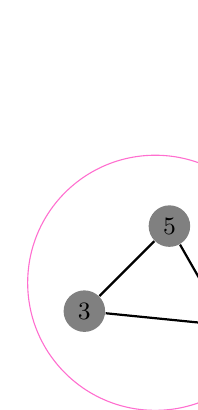
\begin{tikzpicture}[scale=1.8,auto,swap]

            \node[vertex] (1) at (-0.8,1.9) {1};
            \node[vertex] (2) at (3,1.7) {2};
            \node[vertex] (3) at (0.4,0.5) {3};
            \node[vertex] (4) at (-1.2,1.2) {4};
            \node[vertex] (5) at (1,1.1) {5};
            \node[vertex] (6) at (1.4,0.4) {6};
            \node[vertex] (7) at (-1.9,1.7) {7};

            \path[edge] (1) -- (4);
            \path[edge] (4) -- (7);
            \path[edge] (3) -- (5);
            \path[edge] (5) -- (6);
            \path[edge] (6) -- (3);

            \onslide<3->{
                \draw[color=vhilight] (-1.3,1.55) ellipse (0.9cm and 0.9cm);
                \draw[color=vhilight] (0.9,0.7) ellipse (0.9cm and 0.9cm);
                \draw[color=vhilight] (3,1.7) ellipse (0.3cm and 0.3cm);
            }

            \pgfresetboundingbox
            \path [use as bounding box] (0,0) rectangle (1,2.5);
        \end{tikzpicture}
    \end{figure}

    \bi
        \onslide<2->{\item $items = \{1,2,3,4,5,6,7\}$}
        \onslide<3->{\item $collections = \{1,4,7\}, \{2\}, \{3,5,6\}$}
        \onslide<4->{\item \texttt{union(2, 5)}}
    \ei
\end{frame}


\begin{frame}{Disjoint sets in graphs}
    \begin{figure}
        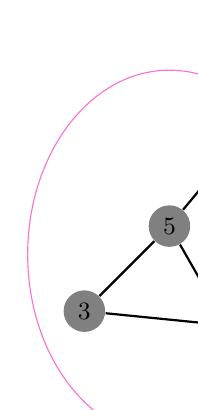
\begin{tikzpicture}[scale=1.8,auto,swap]

            \node[vertex] (1) at (-0.8,1.9) {1};
            \node[vertex] (2) at (1.5,1.7) {2};
            \node[vertex] (3) at (0.4,0.5) {3};
            \node[vertex] (4) at (-1.2,1.2) {4};
            \node[vertex] (5) at (1,1.1) {5};
            \node[vertex] (6) at (1.4,0.4) {6};
            \node[vertex] (7) at (-1.9,1.7) {7};

            \path[edge] (1) -- (4);
            \path[edge] (4) -- (7);
            \path[edge] (3) -- (5);
            \path[edge] (5) -- (6);
            \path[edge] (6) -- (3);
            \path[edge] (2) -- (5);

            \draw[color=vhilight] (-1.3,1.55) ellipse (0.9cm and 0.9cm);
            \draw[color=vhilight] (1.0,0.9) ellipse (1.0cm and 1.3cm);

            \pgfresetboundingbox
            \path [use as bounding box] (0,0) rectangle (1,2.5);
        \end{tikzpicture}
    \end{figure}

    \bi
        \item $items = \{1,2,3,4,5,6,7\}$
        \item $collections = \{1,4,7\}, \{2,3,5,6\}$
        \onslide<2->{\item \texttt{union(6, 2)}}
    \ei
\end{frame}


\begin{frame}{Disjoint sets in graphs}
    \begin{figure}
        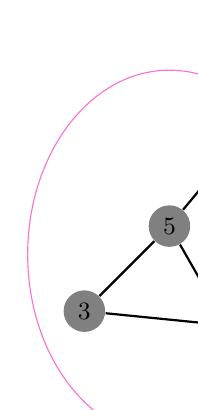
\begin{tikzpicture}[scale=1.8,auto,swap]

            \node[vertex] (1) at (-0.8,1.9) {1};
            \node[vertex] (2) at (1.5,1.7) {2};
            \node[vertex] (3) at (0.4,0.5) {3};
            \node[vertex] (4) at (-1.2,1.2) {4};
            \node[vertex] (5) at (1,1.1) {5};
            \node[vertex] (6) at (1.4,0.4) {6};
            \node[vertex] (7) at (-1.9,1.7) {7};

            \path[edge] (1) -- (4);
            \path[edge] (4) -- (7);
            \path[edge] (3) -- (5);
            \path[edge] (5) -- (6);
            \path[edge] (6) -- (3);
            \path[edge] (2) -- (5);
            \path[edge] (2) -- (6);

            \draw[color=vhilight] (-1.3,1.55) ellipse (0.9cm and 0.9cm);
            \draw[color=vhilight] (1.0,0.9) ellipse (1.0cm and 1.3cm);

            \pgfresetboundingbox
            \path [use as bounding box] (0,0) rectangle (1,2.5);
        \end{tikzpicture}
    \end{figure}

    \bi
        \item $items = \{1,2,3,4,5,6,7\}$
        \item $collections = \{1,4,7\}, \{2,3,5,6\}$
    \ei
\end{frame}

\begin{frame}{Example problem: Friends}
    \bi
        \item http://uva.onlinejudge.org/external/106/10608.html
    \ei
\end{frame}

% TODO: Range queries
\begin{frame}{Range queries}
    \vspace{30pt}
    \bi
        \item We have an array $A$ of size $n$
        \item Given $i,j$, we want to answer:
            \bi
                \item $\mathrm{max}(A[i],A[i+1],\ldots,A[j-1],A[j])$
                \item $\mathrm{min}(A[i],A[i+1],\ldots,A[j-1],A[j])$
                \item $\mathrm{sum}(A[i],A[i+1],\ldots,A[j-1],A[j])$
            \ei
        \item We want to answer these queries efficiently, i.e.\ without looking through all elements
        \item Sometimes we also want to update elements
    \ei
\end{frame}

% TODO: Range sum on a static array
\begin{frame}{Range sum on a static array}
    \bi
        \item Let's look at range sums on a static array (i.e.\ updating is not supported)
    \ei

    \begin{center}
        \begin{tabular}{|c|c|c|c|c|c|c|}
            \hline
            \color<2,3>{vhilight}{1} & \color<2,3>{vhilight}{0} & \color<2,3,4,5,6,7>{vhilight}{7} & \color<2,3,4,5>{vhilight}{8} & \color<2,3,4,5>{vhilight}{5} & \color<2,3,4,5>{vhilight}{9} & \color<2,3>{vhilight}{3} \\
            \hline
        \end{tabular}
    \end{center}

    \bi
        \onslide<2->{\item $\mathrm{sum}(0,6)\onslide<3->{ = 33}$}
        \onslide<4->{\item $\mathrm{sum}(2,5)\onslide<5->{ = 29}$}
        \onslide<6->{\item $\mathrm{sum}(2,2)\onslide<7->{ = 7}$}
        \vspace{20pt}
        \onslide<8->{\item How do we support these queries efficiently?}
    \ei
\end{frame}

\begin{frame}{Range sum on a static array}
    \bi
        \item Simplification: only support queries of the form $\mathrm{sum}(0, j)$
        \item Notice that $\mathrm{sum}(i,j) = \mathrm{sum}(0,j) - \mathrm{sum}(0,i-1)$
    \ei

    \begin{center}
        \begin{tabular}{|c|c|c|c|c|c|c|}
            \hline
            1 & 0 & \color{vhilight}{7} & \color{vhilight}{8} & \color{vhilight}{5} & \color{vhilight}{9} & 3 \\
            \hline
        \end{tabular}
    \end{center}
    $$=$$
    \begin{center}
        \begin{tabular}{|c|c|c|c|c|c|c|}
            \hline
            \color{vhilight}{1} & \color{vhilight}{0} & \color{vhilight}{7} & \color{vhilight}{8} & \color{vhilight}{5} & \color{vhilight}{9} & 3 \\
            \hline
        \end{tabular}
    \end{center}
    $$-$$
    \begin{center}
        \begin{tabular}{|c|c|c|c|c|c|c|}
            \hline
            \color{vhilight}{1} & \color{vhilight}{0} & 7 & 8 & 5 & 9 & 3 \\
            \hline
        \end{tabular}
    \end{center}
\end{frame}

\begin{frame}{Range sum on a static array}
    \bi
        \item So we're only interested in prefix sums
        \item But there are only $n$ of them...
        \item Just compute them all once in the beginning
    \ei

    \begin{center}
        \begin{tabular}{|c|c|c|c|c|c|c|}
            \hline
            1 & 0 & 7 & 8 & 5 & 9 & 3 \\
            \hline
            \onslide<2->{1} & \onslide<3->{1} & \onslide<4->{8} & \onslide<5->{16} & \onslide<6->{21} & \onslide<7->{30} & \onslide<8->{33} \\
            \hline
        \end{tabular}
    \end{center}

    \bi
        \onslide<9->{\item $O(n)$ time to preprocess}
        \onslide<9->{\item $O(1)$ time each query}

        \vspace{10pt}
        \onslide<9->{\item Can we support updating efficiently? \onslide<10->{No, at least not without modification}}
    \ei
\end{frame}

% TODO: Range queries on a dynamic array
\begin{frame}{Range sum on a dynamic array}
    \bi
        \item What if we want to support:
            \bi
                \item sum over a range
                \item updating an element
            \ei
    \ei

    \begin{center}
        \begin{tabular}{|c|c|c|c|c|c|c|}
            \hline
            \color<2,3,6,7>{vhilight}{1} & \color<2,3,6,7>{vhilight}{0} & \color<2,3,6,7>{vhilight}{7} & \color<2,3,4,5,6,7>{vhilight}{\only<-4>{8}\only<5->{-2}} & \color<2,3,6,7>{vhilight}{5} & \color<2,3,6,7>{vhilight}{9} & \color<2,3,6,7>{vhilight}{3} \\
            \hline
        \end{tabular}
    \end{center}

    \bi
        \onslide<2->{\item $\mathrm{sum}(0,6)\onslide<3->{ = 33}$}
        \onslide<4->{\item $\mathrm{update}(3,-2)$}
        \onslide<6->{\item $\mathrm{sum}(0,6)\onslide<7->{ = 23}$}
        \vspace{20pt}
        \onslide<8->{\item How do we support these queries efficiently?}
    \ei
\end{frame}

\begin{frame}[fragile]{Segment Tree}
            \begin{figure}
                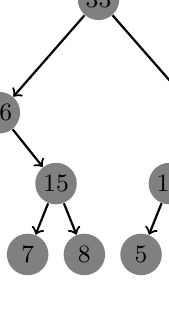
\begin{tikzpicture}[scale=1.8,auto,swap]
                    \onslide<2->{
                        \node[vertex] (0) at (-0.8,0.2) {1};
                        \node[vertex] (1) at (-0.4,0.2) {0};
                        \node[vertex] (2) at (0.0,0.2) {7};
                        \node[vertex] (3) at (0.4,0.2) {8};
                        \node[vertex] (4) at (0.8,0.2) {5};
                        \node[vertex] (5) at (1.2,0.2) {9};
                        \node[vertex] (6) at (1.6,0.2) {3};
                    }

                    \onslide<3->{
                        \node[vertex] (7) at (-0.6,0.7) {1};
                        \node[vertex] (8) at (0.2,0.7) {15};
                        \node[vertex] (9) at (1.0,0.7) {14};
                    }

                    \onslide<4->{
                        \node[vertex] (10) at (-0.2,1.2) {16};
                        \node[vertex] (11) at (1.2,1.2) {17};
                    }

                    \onslide<5->{
                        \node[vertex] (12) at (0.5,2.0) {33};
                    }

                    \onslide<3->{
                        \path[dedge] (7) -- (0);
                        \path[dedge] (7) -- (1);
                        \path[dedge] (8) -- (2);
                        \path[dedge] (8) -- (3);
                        \path[dedge] (9) -- (4);
                        \path[dedge] (9) -- (5);
                    }

                    \onslide<4->{
                        \path[dedge] (10) -- (7);
                        \path[dedge] (10) -- (8);
                        \path[dedge] (11) -- (9);
                        \path[dedge] (11) -- (6);
                    }

                    \onslide<5->{
                        \path[dedge] (12) -- (10);
                        \path[dedge] (12) -- (11);
                    }

                    \pgfresetboundingbox
                    \path [use as bounding box] (0,0) rectangle (0.8,1.8);
                \end{tikzpicture}
            \end{figure}

    \begin{center}
        \begin{tabular}{|c|c|c|c|c|c|c|}
            \hline
                1 & 0 & 7 & 8 & 5 & 9 & 3 \\
            \hline
        \end{tabular}
    \end{center}

    \bi
        \onslide<6>{\item Each vertex contains the sum of some segment of the array}
    \ei
\end{frame}

\begin{frame}[fragile]{Segment Tree - Code}
    \begin{minted}[fontsize=\scriptsize]{cpp}
struct segment_tree {
    segment_tree *left, *right;
    int from, to, value;
    segment_tree(int from, int to)
        : from(from), to(to), left(NULL), right(NULL), value(0) { }
};

segment_tree* build(const vector<int> &arr, int l, int r) {
    if (l > r) return NULL;
    segment_tree *res = new segment_tree(l, r);
    if (l == r) {
        res->value = arr[l];
    } else {
        int m = (l + r) / 2;
        res->left = build(arr, l, m);
        res->right = build(arr, m + 1, r);
        if (res->left != NULL) res->value += res->left->value;
        if (res->right != NULL) res->value += res->right->value;
    }
    return res;
}
    \end{minted}
\end{frame}

\begin{frame}[fragile]{Querying a Segment Tree}
            \begin{figure}
                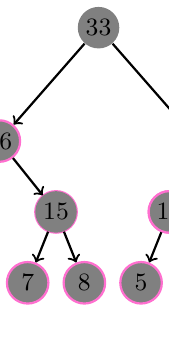
\begin{tikzpicture}[scale=1.8,auto,swap]

                    \onslide<-2,4->{
                        \node[vertex] (0) at (-0.8,0.2) {1};
                        \node[vertex] (1) at (-0.4,0.2) {0};
                        \node[vertex] (2) at (0.0,0.2) {7};
                        \node[vertex] (3) at (0.4,0.2) {8};
                        \node[vertex] (4) at (0.8,0.2) {5};
                        \node[vertex] (5) at (1.2,0.2) {9};
                    }
                    \onslide<3>{
                        \node[selected vertex] (0) at (-0.8,0.2) {1};
                        \node[selected vertex] (1) at (-0.4,0.2) {0};
                        \node[selected vertex] (2) at (0.0,0.2) {7};
                        \node[selected vertex] (3) at (0.4,0.2) {8};
                        \node[selected vertex] (4) at (0.8,0.2) {5};
                        \node[selected vertex] (5) at (1.2,0.2) {9};
                    }
                    \node[vertex] (6) at (1.6,0.2) {3};

                    \onslide<-3>{
                        \node[vertex] (7) at (-0.6,0.7) {1};
                        \node[vertex] (8) at (0.2,0.7) {15};
                        \node[vertex] (9) at (1.0,0.7) {14};
                    }
                    \onslide<4>{
                        \node[selected vertex] (7) at (-0.6,0.7) {1};
                        \node[selected vertex] (8) at (0.2,0.7) {15};
                        \node[selected vertex] (9) at (1.0,0.7) {14};
                    }
                    \onslide<5->{
                        \node[vertex] (7) at (-0.6,0.7) {1};
                        \node[vertex] (8) at (0.2,0.7) {15};
                        \node[selected vertex] (9) at (1.0,0.7) {14};
                    }

                    \onslide<-5>{
                        \node[vertex] (10) at (-0.2,1.2) {16};
                    }
                    \onslide<5->{
                        \node[selected vertex] (10) at (-0.2,1.2) {16};
                    }
                    \node[vertex] (11) at (1.2,1.2) {17};

                    \node[vertex] (12) at (0.5,2.0) {33};

                    \path[dedge] (7) -- (0);
                    \path[dedge] (7) -- (1);
                    \path[dedge] (8) -- (2);
                    \path[dedge] (8) -- (3);
                    \path[dedge] (9) -- (4);
                    \path[dedge] (9) -- (5);

                    \path[dedge] (10) -- (7);
                    \path[dedge] (10) -- (8);
                    \path[dedge] (11) -- (9);
                    \path[dedge] (11) -- (6);

                    \path[dedge] (12) -- (10);
                    \path[dedge] (12) -- (11);

                    \pgfresetboundingbox
                    \path [use as bounding box] (0,0) rectangle (0.8,2.0);
                \end{tikzpicture}
            \end{figure}

    \begin{center}
        \begin{tabular}{|c|c|c|c|c|c|c|}
            \hline
            \color<2->{vhilight}{1} & \color<2->{vhilight}{0} & \color<2->{vhilight}{7} & \color<2->{vhilight}{8} & \color<2->{vhilight}{5} & \color<2->{vhilight}{9} & 3 \\
            \hline
        \end{tabular}
    \end{center}

    \bi
        % \item How do we query the tree?
        \onslide<2->{\item $\mathrm{sum}(0,5)\onslide<6->{= 16 + 14 = 30}$}
        \onslide<7->{\item We only need to consider a few vertices to get the entire range}
        \onslide<8->{\item But how do we find them?}
    \ei
\end{frame}

\begin{frame}[fragile]{Querying a Segment Tree}
            \begin{figure}
                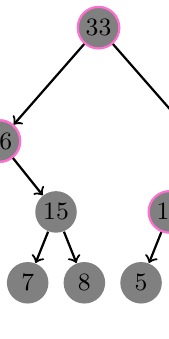
\begin{tikzpicture}[scale=1.8,auto,swap]

                    % \onslide<-2,4->{
                        \node[vertex] (0) at (-0.8,0.2) {1};
                        \node[vertex] (1) at (-0.4,0.2) {0};
                        \node[vertex] (2) at (0.0,0.2) {7};
                        \node[vertex] (3) at (0.4,0.2) {8};
                        \node[vertex] (4) at (0.8,0.2) {5};
                        \node[vertex] (5) at (1.2,0.2) {9};
                    % }
                    % \onslide<3>{
                    %     \node[selected vertex] (0) at (-0.8,0.2) {1};
                    %     \node[selected vertex] (1) at (-0.4,0.2) {0};
                    %     \node[selected vertex] (2) at (0.0,0.2) {7};
                    %     \node[selected vertex] (3) at (0.4,0.2) {8};
                    %     \node[selected vertex] (4) at (0.8,0.2) {5};
                    %     \node[selected vertex] (5) at (1.2,0.2) {9};
                    % }
                    \onslide<-4,6->{
                        \node[vertex] (6) at (1.6,0.2) {3};
                    }
                    \onslide<5>{
                        \node[selected vertex] (6) at (1.6,0.2) {3};
                    }

                    % \onslide<-3>{
                        \node[vertex] (7) at (-0.6,0.7) {1};
                        \node[vertex] (8) at (0.2,0.7) {15};
                    \onslide<-4>{
                        \node[vertex] (9) at (1.0,0.7) {14};
                    }
                    \onslide<5->{
                        \node[selected vertex] (9) at (1.0,0.7) {14};
                    }
                    % }
                    % \onslide<4>{
                    %     \node[selected vertex] (7) at (-0.6,0.7) {1};
                    %     \node[selected vertex] (8) at (0.2,0.7) {15};
                    %     \node[selected vertex] (9) at (1.0,0.7) {14};
                    % }
                    % \onslide<5->{
                    %     \node[vertex] (7) at (-0.6,0.7) {1};
                    %     \node[vertex] (8) at (0.2,0.7) {15};
                    %     \node[selected vertex] (9) at (1.0,0.7) {14};
                    % }

                    \onslide<-3>{
                        \node[vertex] (10) at (-0.2,1.2) {16};
                        \node[vertex] (11) at (1.2,1.2) {17};
                    }
                    \onslide<4>{
                        \node[selected vertex] (10) at (-0.2,1.2) {16};
                        \node[selected vertex] (11) at (1.2,1.2) {17};
                    }
                    \onslide<5->{
                        \node[selected vertex] (10) at (-0.2,1.2) {16};
                        \node[vertex] (11) at (1.2,1.2) {17};
                    }

                    \onslide<-2,4->{
                        \node[vertex] (12) at (0.5,2.0) {33};
                    }
                    \onslide<3>{
                        \node[selected vertex] (12) at (0.5,2.0) {33};
                    }

                    \path[dedge] (7) -- (0);
                    \path[dedge] (7) -- (1);
                    \path[dedge] (8) -- (2);
                    \path[dedge] (8) -- (3);
                    \path[dedge] (9) -- (4);
                    \path[dedge] (9) -- (5);

                    \path[dedge] (10) -- (7);
                    \path[dedge] (10) -- (8);
                    \path[dedge] (11) -- (9);
                    \path[dedge] (11) -- (6);

                    \path[dedge] (12) -- (10);
                    \path[dedge] (12) -- (11);

                    \pgfresetboundingbox
                    \path [use as bounding box] (0,0) rectangle (0.8,2.0);
                \end{tikzpicture}
            \end{figure}

    \begin{center}
        \begin{tabular}{|c|c|c|c|c|c|c|}
            \hline
            \color<2->{vhilight}{1} & \color<2->{vhilight}{0} & \color<2->{vhilight}{7} & \color<2->{vhilight}{8} & \color<2->{vhilight}{5} & \color<2->{vhilight}{9} & 3 \\
            \hline
        \end{tabular}
    \end{center}

    \bi
        \item $\mathrm{sum}(0,5)$
    \ei
\end{frame}

\begin{frame}[fragile]{Querying a Segment Tree - Code}
    \vspace{50pt}
    \begin{minted}[fontsize=\scriptsize]{cpp}
int query(segment_tree *tree, int l, int r) {
    if (tree == NULL) return 0;
    if (l <= tree->from && tree->to <= r) return tree->value;
    if (tree->to < l) return 0;
    if (r < tree->from) return 0;
    return query(tree->left, l, r) + query(tree->right, l, r);
}
    \end{minted}
\end{frame}


\begin{frame}[fragile]{Updating a Segment Tree}
    \begin{figure}
        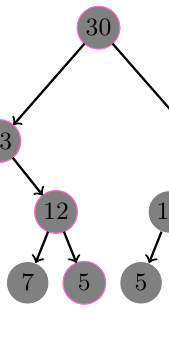
\begin{tikzpicture}[scale=1.8,auto,swap]
            \node[vertex] (0) at (-0.8,0.2) {1};
            \node[vertex] (1) at (-0.4,0.2) {0};
            \node[vertex] (2) at (0.0,0.2) {7};
            \onslide<-2>{
                \node[vertex] (3) at (0.4,0.2) {8};
            }
            \onslide<3>{
                \node[selected vertex] (3) at (0.4,0.2) {8};
            }
            \onslide<4>{
                \node[selected vertex] (3) at (0.4,0.2) {5};
            }
            \onslide<5->{
                \node[vertex] (3) at (0.4,0.2) {5};
            }
            \node[vertex] (4) at (0.8,0.2) {5};
            \node[vertex] (5) at (1.2,0.2) {9};
            \node[vertex] (6) at (1.6,0.2) {3};

            \node[vertex] (7) at (-0.6,0.7) {1};
            \onslide<-4>{
                \node[vertex] (8) at (0.2,0.7) {15};
            }
            \onslide<5>{
                \node[selected vertex] (8) at (0.2,0.7) {15};
            }
            \onslide<6>{
                \node[selected vertex] (8) at (0.2,0.7) {12};
            }
            \onslide<7->{
                \node[vertex] (8) at (0.2,0.7) {12};
            }
            \node[vertex] (9) at (1.0,0.7) {14};

            \onslide<-6>{
                \node[vertex] (10) at (-0.2,1.2) {16};
            }
            \onslide<7>{
                \node[selected vertex] (10) at (-0.2,1.2) {16};
            }
            \onslide<8>{
                \node[selected vertex] (10) at (-0.2,1.2) {13};
            }
            \onslide<9->{
                \node[vertex] (10) at (-0.2,1.2) {13};
            }
            \node[vertex] (11) at (1.2,1.2) {17};

            \onslide<-8>{
                \node[vertex] (12) at (0.5,2.0) {33};
            }
            \onslide<9>{
                \node[selected vertex] (12) at (0.5,2.0) {33};
            }
            \onslide<10>{
                \node[selected vertex] (12) at (0.5,2.0) {30};
            }
            \onslide<11->{
                \node[vertex] (12) at (0.5,2.0) {30};
            }

            \path[dedge] (7) -- (0);
            \path[dedge] (7) -- (1);
            \path[dedge] (8) -- (2);
            \path[dedge] (8) -- (3);
            \path[dedge] (9) -- (4);
            \path[dedge] (9) -- (5);

            \path[dedge] (10) -- (7);
            \path[dedge] (10) -- (8);
            \path[dedge] (11) -- (9);
            \path[dedge] (11) -- (6);

            \path[dedge] (12) -- (10);
            \path[dedge] (12) -- (11);

            \pgfresetboundingbox
            \path [use as bounding box] (0,0) rectangle (0.8,2.0);
        \end{tikzpicture}
    \end{figure}

    \begin{center}
        \begin{tabular}{|c|c|c|c|c|c|c|}
            \hline
            1 & 0 & 7 & \color<3->{vhilight}{\only<-3>{8}\only<4->{5}} & 5 & 9 & 3 \\
            \hline
        \end{tabular}
    \end{center}

    \bi
        \onslide<2->{\item $update(3, 5)$}
    \ei
\end{frame}

\begin{frame}[fragile]{Updating a Segment Tree - Code}
    \vspace{40pt}
    \begin{minted}[fontsize=\scriptsize]{cpp}
int update(segment_tree *tree, int i, int val) {
    if (tree == NULL) return 0;
    if (tree->to < i) return tree->value;
    if (i < tree->from) return tree->value;
    if (tree->from == tree->to && tree->from == i) {
        tree->value = val;
    } else {
        tree->value = update(tree->left, i, val) + update(tree->right, i, val);
    }
    return tree->value;
}
    \end{minted}
\end{frame}

\begin{frame}{Segment Tree}
    \bi
        \item Now we can
            \bi
        \item build a Segment Tree\onslide<3->{ in {\color{hilight}{$O(n)$}}}
        \item query a range\onslide<4->{ in {\color{hilight}{$O(\log n)$}}}
        \item update a single value\onslide<5->{ in {\color{hilight}{$O(\log n)$}}}
            \ei
        \onslide<2->{\item But how efficient are these operations?}
        \vspace{20pt}
        \onslide<6->{\item Trivial to use Segment Trees for $\min$, $\max$, $\gcd$, and other similar operators, basically the same code}
        \onslide<7->{\item Also possible to update a range of values in $O(\log n)$ (Google for Segment Trees with Lazy Propagation if you want to learn more)}
    \ei
\end{frame}

\begin{frame}{Example problem: Potentiometers}
    \bi
        \item http://uva.onlinejudge.org/external/120/12086.html
    \ei
\end{frame}

% TODO: decide if we should talk about Fenwick Trees
% TODO: Fenwick trees
% \begin{Fenwick Tree}{}

% TODO: Example problems
% \begin{frame}{Example problem: TODO}
%     \bi
%         \item TODO
%     \ei
% \end{frame}

\end{document}

